% !TEX root = ../main.tex

% 第一章一般名为绪论/引言,不可省略

\chapter{本文基础路线}

\section{研究背景}

人工智能与机器学习主要研究的是如何使计算机能够像人类一样思考、决策、行动, 这是计算机科学家们长久以来一直在进行探索的问题。\cite{AIMD} 从20世纪六十年代, 科研工作者普遍关心的是如何利用计算机解决听觉、视觉、语言理解、自动推理等问题。 但是这些问题,尤其是计算机视觉和语音识别问题, 在相当长的一段时间内发展缓慢。 这是因为, 基于之前以分析为主的方法, 例如基于边缘检测等人工主观判断的特征进行图像识别, 或者利用语言学的专家知识进行语义理解和语音识别。 自从1980年,统计概率模型逐渐取代了之前基于规则的算法模型, 其算法的稳定性和泛化性能比起之前基于规则的算法进步很大。 \cite{50_years_ai} \cite{manning2008introduction} \cite{abelson1985structure}

1986年, Geoffery Hinton在Nature杂志上发表了一种利用反向传播(Back Propagation)自动优化神经网络模型的方法, 该方法利用神经网络进行机器学习第二次成为机器学习研究的重点。 在1997年,YaLeCun提出的卷积神经网络(Convolutional Neural Networks)能够识别手写的阿拉伯数字, 这在计算机尤其是人工智能领域是很重要的进步。 但是, 神经网络的参数多, 为了使得其参数收敛至稳定值, 需要大量的训练样本而且其巨大的矩阵运算是一般的计算机所不能承受的, 神经网络虽然有了一些优秀的表现, 但是并没有产生突破性的表现。 

2012年ImageNet计算机视觉识别比赛中,在加拿大蒙特利尔大学担任教授的Geoffery Hinton带领团队使得ImageNet图像识别的错误率由30\%以上下降到15\%一下, 这引起了轰动。 \cite{DBLP:journals/corr/abs-1301-3781} 
% htbp 什么的现在不要管
\begin{figure}[htbp]
    \centering  % 学位论文规定图表皆水平居中于版心 在 zjuthesis.cls 搜「版心设置」
    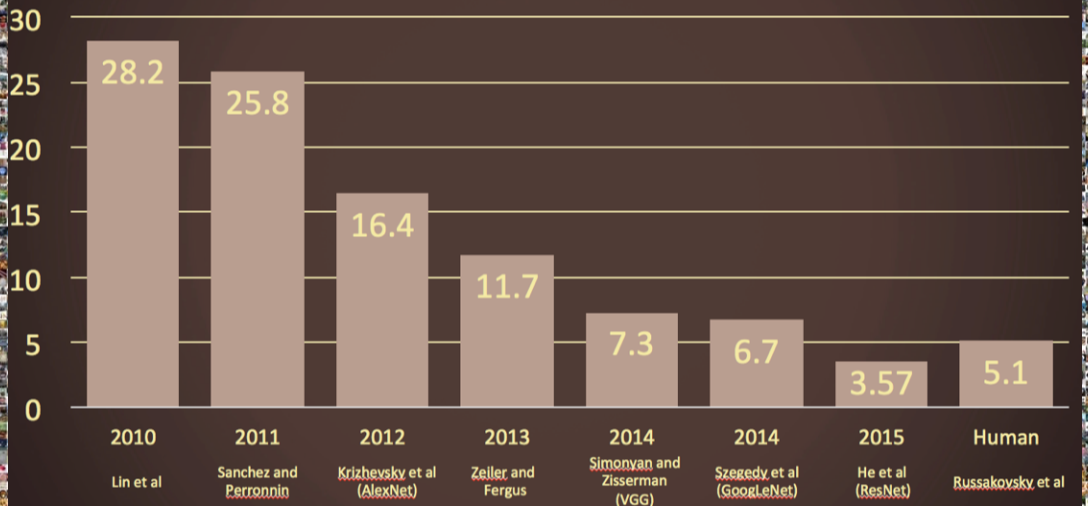
\includegraphics[width = .85\linewidth]{data/chapter-2/image_net_rank.png} % 设定图片宽度相对于版心宽度,图片文件资源名
    \caption{ImageNet 错误率的下降} % 图的题注
    \label{Russakovsky et al. arXiv, 2014} % 与 autoref 关联,设定交叉引用和显示「图x.x」
\end{figure}


从2012年之后, 深度学习这一机器学习范式, 被用来解决诸多问题。 例如此前的ImageNet下进行的计算机视觉比赛, 在2015年其识别的错误率已经低于人类的平均值。 2017年12月22日, 腾讯DPDAC NLP实验室使用深度学习神经网络训练的自然语言理解模型, 在机器阅读理解的比赛上的正确率已经达到81.790\%, 人类在这项测试中的评价准确率为\%82.304。 除计算机视觉和自然语言理解领域, 深度学习在决策领域也表现出了惊人的进步, 2017年10月, Google Deep Mind的AlphGo战胜了战胜了围棋世界排名第一的柯洁, 这表明深度学习在复杂决策上也是具有非常大的潜力。 

由于深度学习在计算机视觉、自然语言理解、决策等方面的突出表现。 科研工作者希望利用深度学习能够解决更加类似于人类的工作, 即 -- 艺术创作。 艺术创作长期以来被认为是人类独有的能力。 但是经过科学家们对于艺术创作过程以及艺术创作心理学的分析发现, 人类的艺术创作除了精神与心理学等生理原因, 其后天影响, 周围环境影响对艺术创作也是具有非常大的影响。 或者说, 创意, 创造力和后天学习具有密不可分的关系。 \cite{mq-zhanjian} \cite{adomavicius2005toward} \cite{gil2010state}

另外, 艺术创作在某些环境下也是重复的脑力活动, 例如在游戏音乐配乐, 游戏场景绘画, 电影场景绘画以及畅销书的写作等。 其重复的模式非常之多。 在此模型下, 艺术创作可以抽象为一个制作或者生成过程,如方程\eqref{eq:gene-art}所示。 

\begin{equation}\label{eq:gene-art}
ArtWork= Generator(f_0, f_1, f_2, \cdots, f_N, r_{x \sim p})
\end{equation} 

但是由于艺术生成具有区别于传统机器学习的两个特点, 第一是:其输出是一个序列性的而非特点长度的标签(Label)或者回归预测值; 第二是: 艺术的输入特征难以确定, 其输入也是一个复杂的序列过程。 例如音乐的生成依赖于诸多因素。 以上两个因素使得计算机进行自动艺术创作, 在长时间内依赖于规则,这使得计算机艺术创作不能广泛得适用于更加通用的场景。 

然而深度学习在特征自动学习(Representation Learning )和序列数据特征的提取中均具有良好的效果。 故,很多科研工作者开始使用深度学习相关的方法来尝试计算机自动生成艺术作品。 

色彩配图是在设计领域长期存在的问题,该任务相较于纯粹的艺术创作,具有较强的重复性。在设计师设计的过程中, 例如设计服饰,软装设计, 建筑外观设计等, 其依据现有的环境特点,应用场景,需要为其艺术线稿进行配色。由于自然语言理解与图像识别等领域目前都有了长足的进步, 所以设计作品自动配色这个问题目前有可能使用神经网络和深度学习的内容进行自动化。 

而且, 由于自然语言理解在最近几年取得的成果, 其在语义理解方面可以良好的应用于设计作品自动配色这样领域。 目前, 设计师们的工作方式是采用一张配色表, 使用关键词进行配色, 例如图 \ref{img:peise} 这种方式进行。 这种方式其实是计算机语言理解的时候的一种折中做法。 

\begin{figure}[htbp]
    \centering  % 学位论文规定图表皆水平居中于版心 在 zjuthesis.cls 搜「版心设置」
    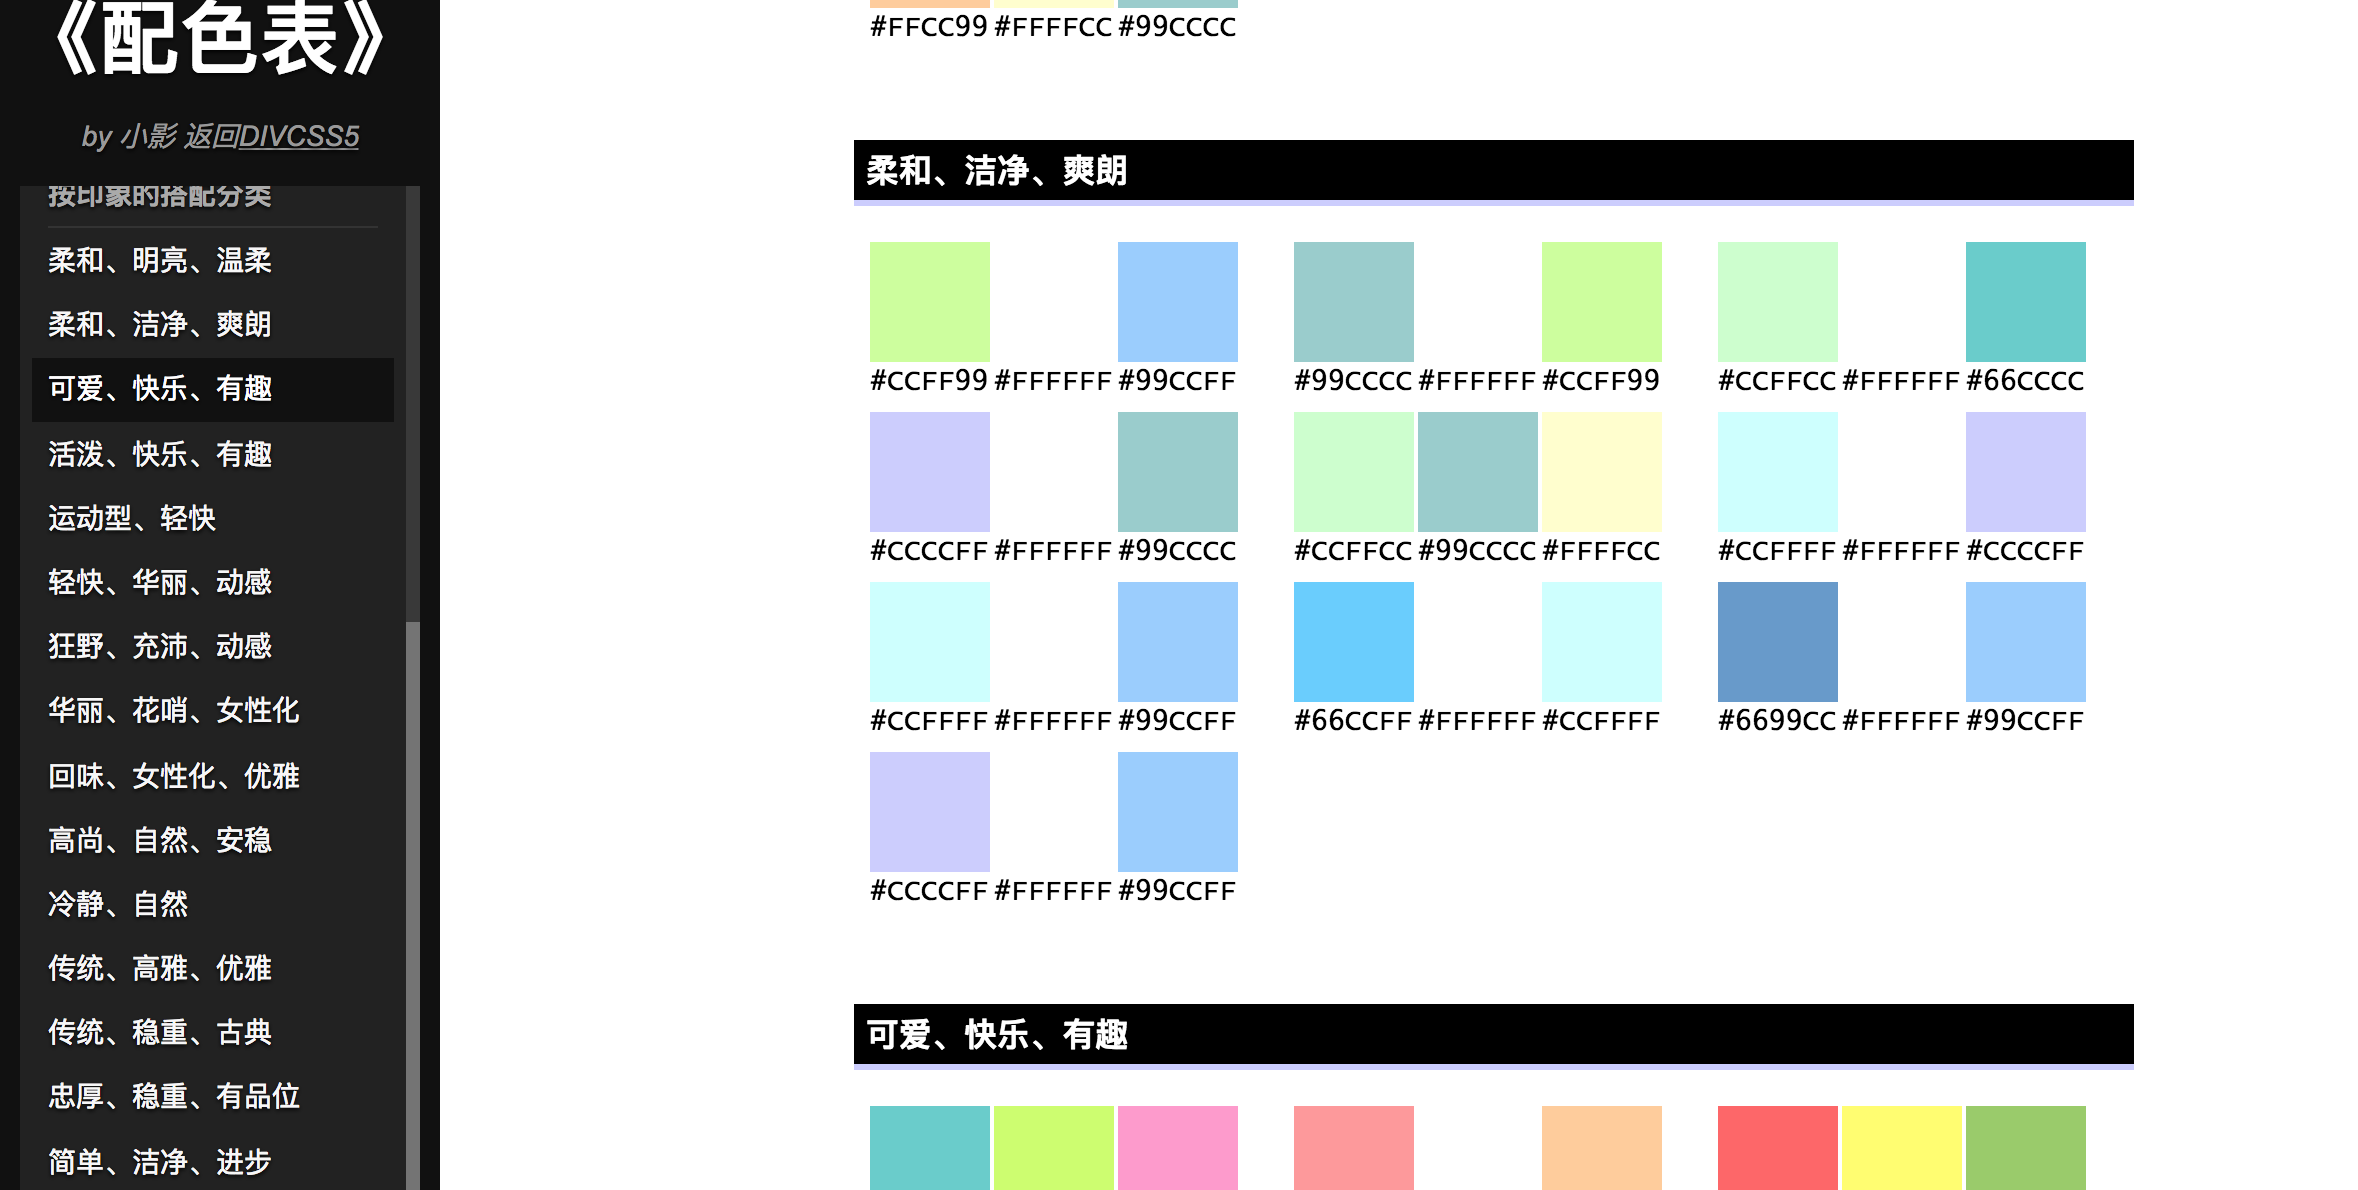
\includegraphics[width = .55\linewidth]{data/chapter-2/peisebiao.png} % 设定图片宽度相对于版心宽度,图片文件资源名
    \caption{设计师使用配色表进行配色} % 图的题注
    \label{img:peise} % 与 autoref 关联,设定交叉引用和显示「图x.x」
\end{figure}

这种方式存在两个问题:第一, 有限的词汇其实不能表达丰富的含义,设计作品的应用涵盖生活的方方面面, 其需要表达的语义丰富性是远远高于有限的这些单词的; 第二,单个词汇与整体意向组织不具备线性叠加的关系。 即, 设计师要设计出一个“温柔的春天”这样意境的设计作品, 其颜色不能是先选择“温柔”, 再选择“春天”, 而是需要再次进行加工。 将这两种的意向进行重叠。 而这种加工是目前的配色表不能完成的。 

因此, 本课题希望基于目前的自然语言理解的技术与图像自动化处理的方式, 实现从作者的直接描述到自动产生配色图的自动化转化。 例如, 一个设计师接到了室内软装设计的需求, 甲方的需求是\textbf{“洋溢着春天的感觉, 要很温柔, 然后要像有小孩在草坪上奔跑一样”}, 本课题要实现的, 设计师只需要关注其设计稿, 最后的配色, 只需要将这句话\textbf{“洋溢着春天的感觉, 要很温柔, 然后要像有小孩在草坪上奔跑一样”},输入到系统中, 就会自动为其线稿进行配色。 

而本文之上的分析, 本课题研究一种例如深度学习与表示学习的方式, 在此基础上实现从语言理解到色彩搭配的自动转化。 之后, 本课题在真实数据库上进行了实验, 本模型确实能够实现良好的自动化转化, 证明了该模型的有效性。 


\section{国内外研究现状}

因为本研究课题是机器学习、自然语言处理和图像合成的交叉领域, 本小节主要从以下三方面进行国内外现状的分析: 

\begin{enumerate}

	\item 自动图像合成
	\item 表示学习 (Representation Learning)
	\item 序列化生成 
	
\end{enumerate}

\subparagraph{计算机自动图像生成} 实现计算机自动图像生成或自动色彩搭配,目前涉及到的方法如下: 

\begin{itemize}

	\item 查表法
	\item 马尔可夫链
	\item 机器学习与人工智能方法
	\item 原细胞有限自动机
	\item 基于规则的算法 [Wiggins(1991), Nierhaus(2009)]
	
\end{itemize}

%除使用以上方法, 目前仍有人工定义负责算法进行音乐的自动合成, 例如Wiggins(1991), Nierhaus(2009)。 

使用机器学习与人工智能方法主要分为两个类型, 一是监督式的(Supervised), 希望给计算机一定的监督样本(Samples), 使得计算机能够拟合一个函数, 使得该函数能够拟合训练数据到已知样本标签的映射如等式 \eqref{eq:map}

\begin{equation}\label{eq:map}
function(x) \rightarrow y
\end{equation}

监督式的学习方式在图像生成领域应用不多, 主要使用因为该种方式主要应用在问题结果确定已知并且有限的情况下, 即 其目标函数的$y in \mathbf{R}^n$ 且 $|y| <= N$ 。 但是, 图像生成领域,目标函数的结果大家的期望并不是从已知的范围内选择一些出来,而是希望能够自动创作。 

所以目前机器学习方式主要采用\textbf{非监督学习}的方式进行图像生成。 非监督的学习方式主要通过从已知的信息中, 获得不同类型的信息、数据的隐含关系, 例如图 \ref{img:unsupervised}。 

\begin{figure}[htbp]
    \centering  % 学位论文规定图表皆水平居中于版心 在 zjuthesis.cls 搜「版心设置」
    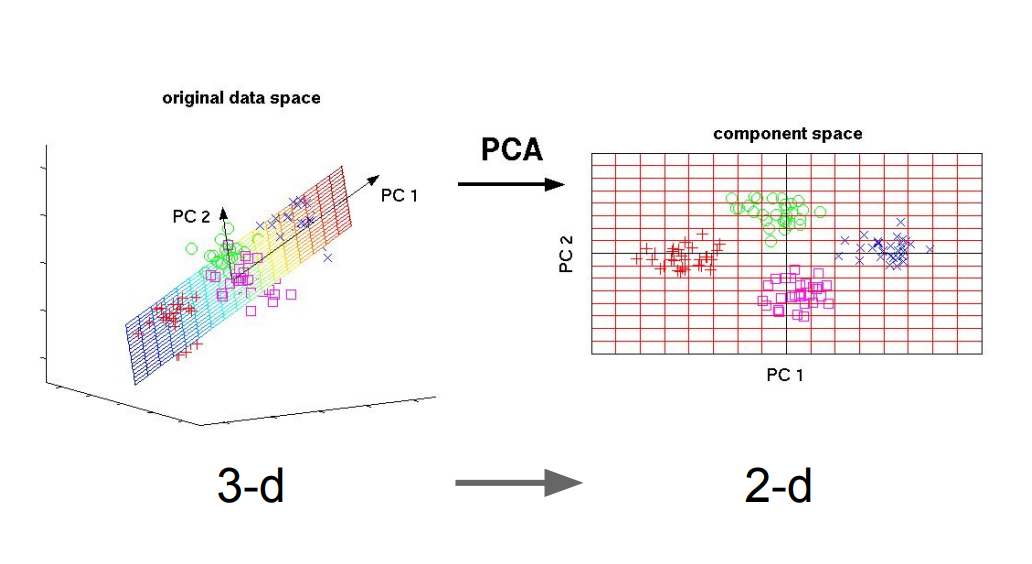
\includegraphics[width = .55\linewidth]{data/chapter-2/unsupervised.png} % 设定图片宽度相对于版心宽度,图片文件资源名
    \caption{非监督式学习主要用来找到影藏的关系} % 图的题注
    \label{img:unsupervised} % 与 autoref 关联,设定交叉引用和显示「图x.x」
\end{figure}

而基于非监督是的学习, 提出的Autoencoder \cite{} 自编码模型可以在缺少某些信息的情况下, 对图像进行重建。 例如图 \ref{img:autoencoder} 所示。

\begin{figure}[htbp]
    \centering  % 学位论文规定图表皆水平居中于版心 在 zjuthesis.cls 搜「版心设置」
    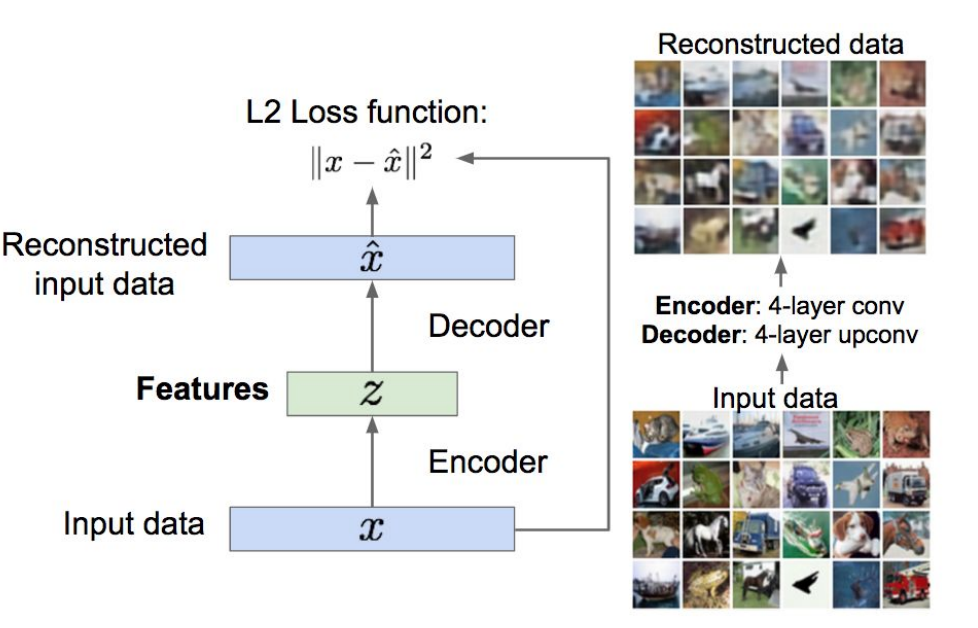
\includegraphics[width = .55\linewidth]{data/chapter-2/autoencoder.png} % 设定图片宽度相对于版心宽度,图片文件资源名
    \caption{自编码模型可以从缺少的信息中重建图片} % 图的题注
    \label{img:autoencoder} % 与 autoref 关联,设定交叉引用和显示「图x.x」
\end{figure}

由于重建信息的成功, 如图 \ref{img:autoencoder}, 科研人员考虑如何通过已知的数据, 获得其潜在的数据概率分布, 从而可以不依靠部分信息而对全部的信息进行重建, 以重建其具备与源数据源具有同样数据分布的数据。 

\begin{figure}[htbp]
    \centering  % 学位论文规定图表皆水平居中于版心 在 zjuthesis.cls 搜「版心设置」
    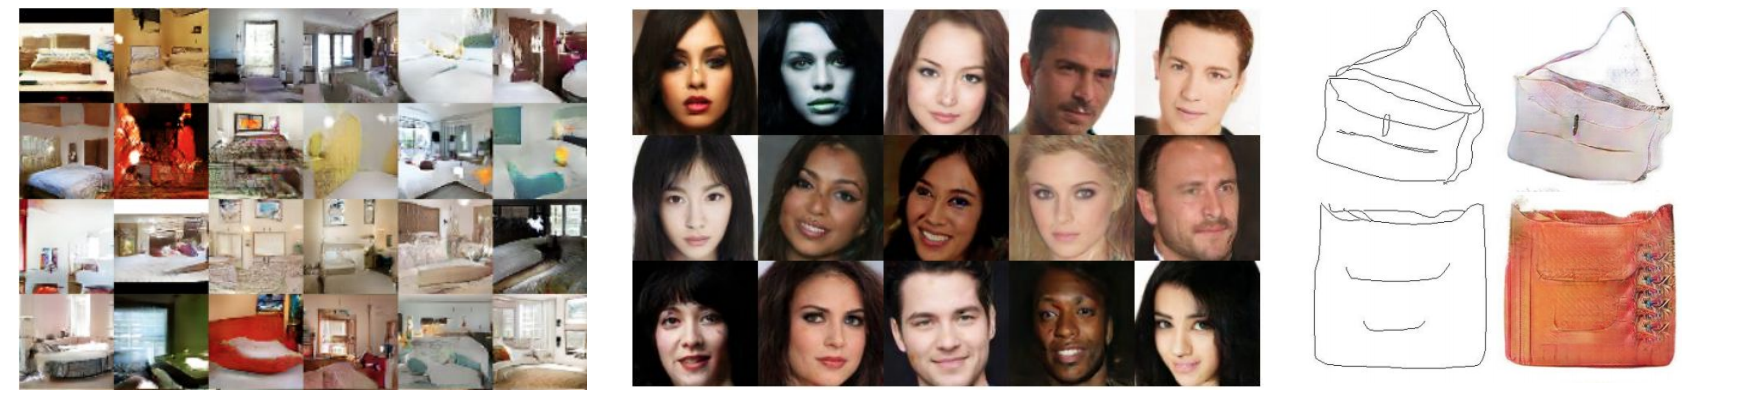
\includegraphics[width = .55\linewidth]{data/chapter-2/gene.png} % 设定图片宽度相对于版心宽度,图片文件资源名
    \caption{生成模型可以直接生成新的信息而不基于输入的部分信息} % 图的题注
    \label{img:gene} % 与 autoref 关联,设定交叉引用和显示「图x.x」
\end{figure}

要完成此任务, 目前主流的使用PixelRNN/CNN, GAN,马尔科夫连, 以及模仿学习(Imitation Learning), 这些模型都可以模型训练之后, 不需要输入部分“初始信息”, 而直接获得新的符合原来数据分布的新数据, 例如图 \ref{img:gene} 所示, 模型可以随机的产生室内的图片, 人像, 以及自动为线稿配色。  

要达到此效果,常见的方式有以下几种

\begin{enumerate}
\item{\textbf{PixelRNN/CNN}}
\item{\textbf{GAN}}
\item{\textbf{马尔可夫链}}
\item{\textbf{模仿学习(Imitation Learning)}}
\end{enumerate}

\subsection{PixelRNN/CNN}

\begin{equation}\label{eq:pix}
p(x) = \prod_{i=n}^{n} p(x_i|x1, ..., x_{i-1})
\end{equation}

该模型基于一个信念网络(Belief network) \eqref{eq:pix}, 其中, $ p(x) $ 是某图像 $x$ 的似然分布, 而 $pr(x_i|x_1, ..., x_{i-1}$ 是某个像素的概率在给定该像素之前的所以像素分布之下的条件概率。 该信念网络希望通过网络模型获得其条件概率的最大分布。 要生成一个像素 pixel 需要获得上一个 pixel的值, 通过一个RNN或者CNN网络, 实现序列化的生成, 如图 \ref{img:pix-matrix} 所示。 

\begin{figure}[htbp]
    \centering  % 学位论文规定图表皆水平居中于版心 在 zjuthesis.cls 搜「版心设置」
    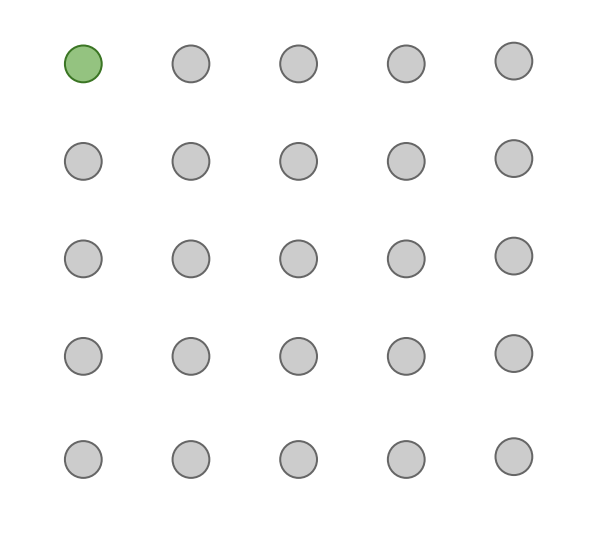
\includegraphics[width = .55\linewidth]{data/chapter-2/pixel_matrix.png} % 设定图片宽度相对于版心宽度,图片文件资源名
    \caption{pixel network 通过序列化的像素生成图像} % 图的题注
    \label{img:pix-matrix} % 与 autoref 关联,设定交叉引用和显示「图x.x」
\end{figure}

依照此模型, 可以自动生成图像, 例如图 \ref{img:pix-example} 所示, 该模型在进行CFAIR10和ImageNet数据库的训练之后, 能够随机生成与之类似的图形. 

\begin{figure}[htbp]
    \centering  % 学位论文规定图表皆水平居中于版心 在 zjuthesis.cls 搜「版心设置」
    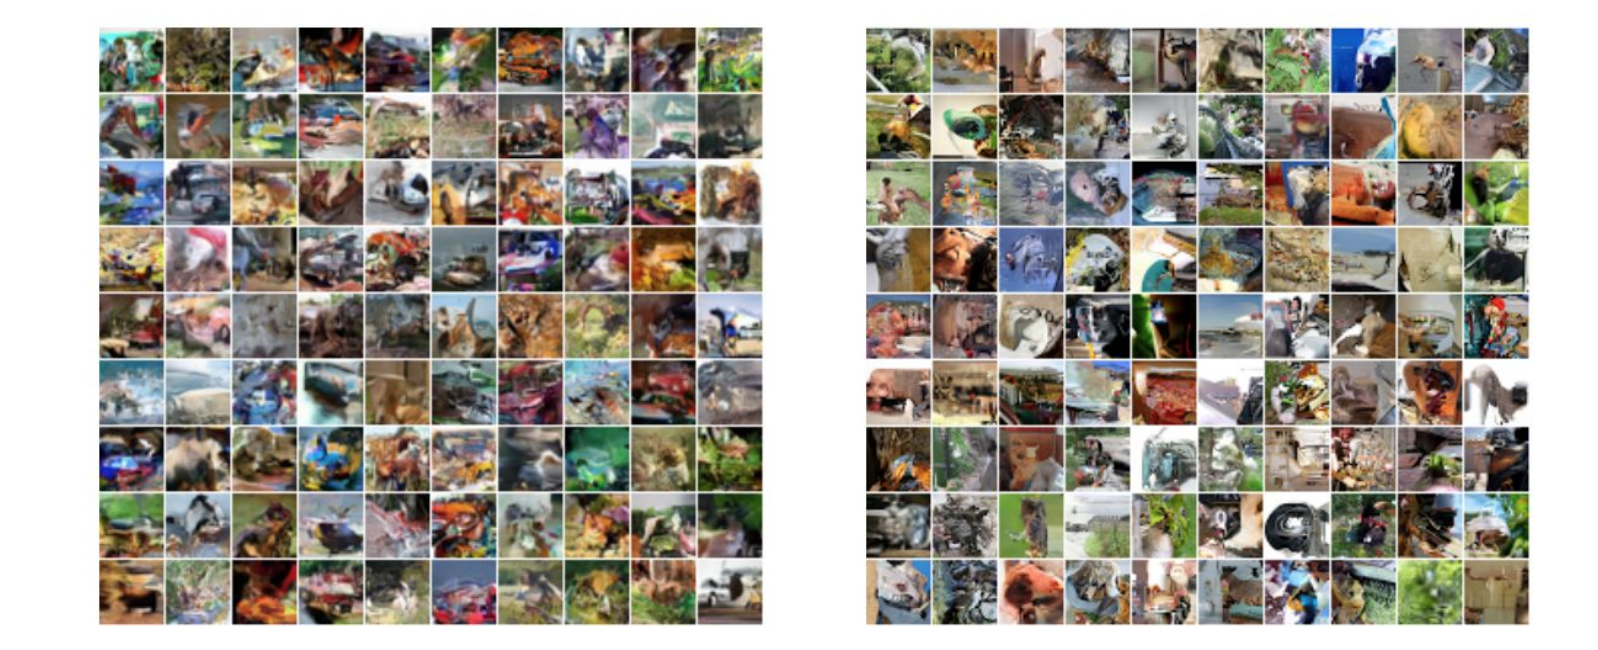
\includegraphics[width = .55\linewidth]{data/chapter-2/pixel_example.png} % 设定图片宽度相对于版心宽度,图片文件资源名
    \caption{pixel network 通过序列化的像素生成图像} % 图的题注
    \label{img:pix-example} % 与 autoref 关联,设定交叉引用和显示「图x.x」
\end{figure}



\subparagraph{表示学习与Embedding} 表示学习是机器学习中重要的研究内容, 主要研究如何将数据有效的表示到计算机中。 其中, 最重要的的方式是如何通过一种方式使得新表现的数据形式能够保持其原始线性关系\cite{embedding}, 这种行为在计算机及数学中叫做embedding。Embedding是指,保持一种偏序关系,是的我们已知的某种关系也保持到新的向量空间中。 Embedding的具体定义如下:

$$ \forall x_{1},x_{2}\in X:x_{1}\leq x_{2}\Leftrightarrow F(x_{1})\leq F(x_{2}). $$


例如,之前人们对自然语言进行计算的时候, 使用的表示方式多是one-hot方法表示单词或者利用tf-idf等信息表示一句话。 但是这种表示并不能表征有效的表征句意。 Mikolov 等科学家使用的word2vec, 使得我们能够获得更加深层次的语义 \cite{DBLP:journals/corr/abs-1301-3781}。 由于word2vec保持了词汇意思的线性关系, 使得我们利用已知的单词获得新的,意思解决的单词变成了可能。 在Mikolov提出了Skip-Gram和CBOW等word Embedding的方法之后, 斯坦福大学NLP组提出的Glove,以及Salesforce提出的ContexVec \cite{DBLP:journals/corr/abs-1708-00107} 都获得更加良好的表现。 


\begin{figure}[htbp]
    \centering  % 学位论文规定图表皆水平居中于版心 在 zjuthesis.cls 搜「版心设置」
    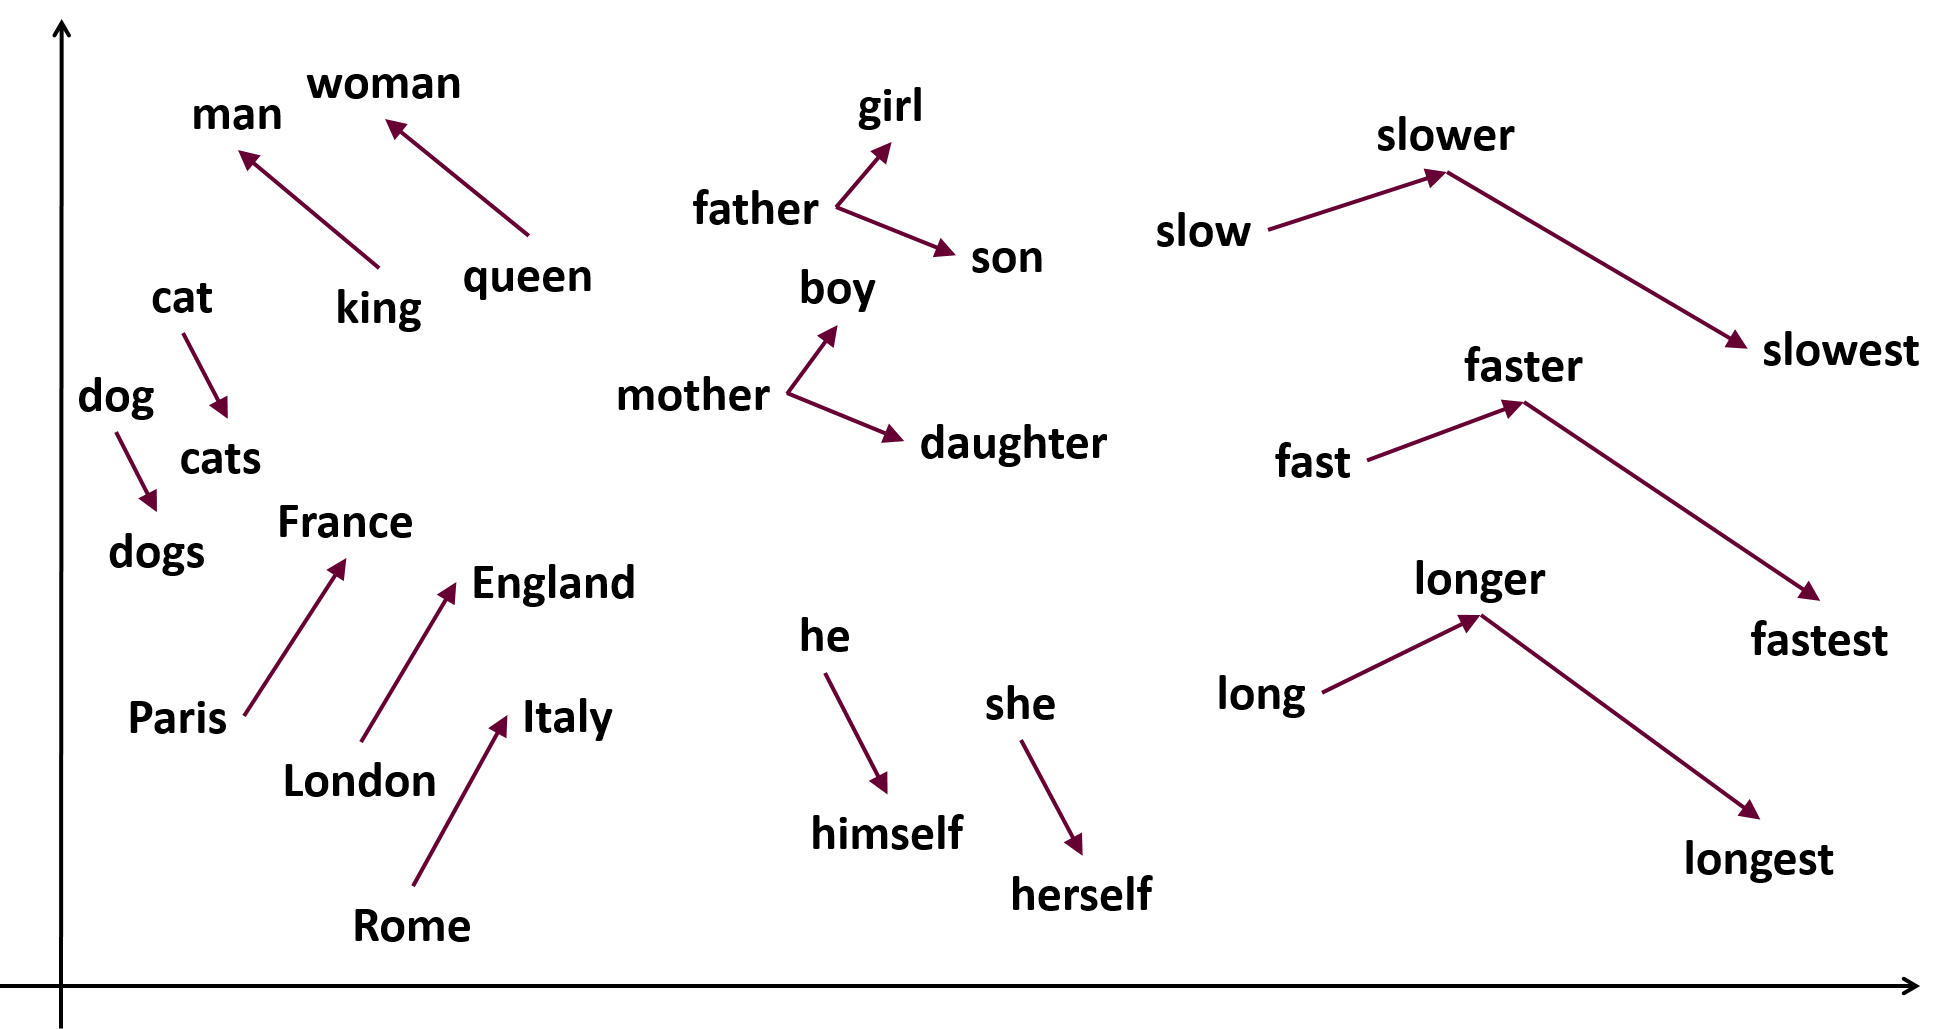
\includegraphics[width = .85\linewidth]{data/chapter-2/word2vec2.png} % 设定图片宽度相对于版心宽度,图片文件资源名
    \caption{Word Embedding 对单词词义的线性保持} % 图的题注
    \label{word2vec} % 与 autoref 关联,设定交叉引用和显示「图x.x」
\end{figure}

本文借鉴 word embedding 的思想,对音乐元素进行embedding, 这样做的好处是, 将以前的88个音乐元素扩展至用户可自定义的个数个音乐元素(依照训练数据的不同, 该自定义元素数字可从几千至几十万), 这些音乐元素经过embedding, 可使得具有类似情感,类似表达的音乐元素进行聚类。 让计算机把音乐元素当做88个单独的元素看待类似于让计算机把所有的英文文本当做26个字母看待。 经过以上关于word embdding的分析, 这显然是低效的。 如果能够让计算机自动发现类似于单词的音乐元素词组, 将能够大大提示模型的抽象能力与泛化能力。 


\section{论文研究内容}

文论文主要研究以下内容:

\begin{itemize}

	\item{如何获得大量的音乐训练数据}
	\item{如何高效的进行音乐元素的embedding}
	\item{如何构建序列生成模型}
	\item{如何将模型迁移适应到古代诗歌风格}

\end{itemize}


\section{论文组织结构}

%简明扼要的介绍下各章主旨,版面控制半页内。

\begin{itemize}

\item 第二章 \textbf{音乐元素的表征和embedding}

第二章主要解决如何将音乐元素进行有效的表征和embedding, 主要涉及到音乐元素的离散化、正则化以及标准化。 这是使得模型能够有效利用数据进行结果输出。 

\item 第三章 \textbf{歌词词向量的构建}

第三章主要利用word2vec的方法将所有的歌词进行向量化, 这是模型能够有效的使用输入训练数据进行学习。

\item 第四章 \textbf{训练数据的生成}

依据前文生成的音乐向量以及词向量, 可以此基础之上构建训练数据。 通过N-Gram滑窗, Skip-Gram随机跳跃, 以及利用word2vec结果进行同义词替换等方法, 使得模型获得了大量的训练数据。 


\item 第五章 \textbf{计算机序列生成模型的构建}

此章研究使用Seq2Seq进行序列生成的原因以及如何将Seq2Seq利用到该课题中。 主要解决此问题范式是否为可学习、可训练的问题, 以及如何使得该问题变成可学习,可训练的问题。 如何设计网络结构,层级结构, 如何选择神经元, 如何设计Loss函数, 如何设计输出输入格式, 使得该模型可训练。 

\item 第六章 \textbf{系统模型实现与结果分析}

通过网易云音乐下载的1000首歌曲, 以及通过编写网络爬虫从网络中获取到的这1000首歌曲匹配的歌词。 在此模型上进行训练,观察实验结果。 并且通过对训练结过程及结果的分析, 获得此模型的学习能力及泛化效果。 

%\item 第七章 \textbf{针对《诗经》的迁移训练}

%此章讨论如何利用迁移学习将此模型迁移到适用于《诗经》的歌曲生成中。 

\item 第七章 \textbf{总结分析}

此章讨论了此模型的优点和存在的问题, 以及提出了对未来的展望。 

\end{itemize}
